\documentclass{article}
\usepackage{amsmath}
\usepackage{amssymb}
\usepackage{graphicx}
\usepackage{tikz}
\usepackage{pgfplots}
\pgfplotsset{compat=1.18}
\usepackage{booktabs}
\usepackage{xcolor}

% Custom environments as required
\newenvironment{lesson-meta}{}{}
\newenvironment{item-analysis}{}{}
\newenvironment{model-discuss}{}{}
\newenvironment{concept-box}{}{}
\newenvironment{concept-summary}{}{}
\newenvironment{example}[1]{\textbf{EXAMPLE #1}}{}
\newenvironment{tryit}[1]{\textbf{Try It! #1}}{}
\newenvironment{practice}[2]{\textbf{#1.}}{}
\newenvironment{te-addendum}[2]{}{}
\newcommand{\answer}[1]{}
\newcommand{\placeholder}[2]{[#1: #2]}
\newcommand{\uncertain}[2]{#1}
\newcommand{\te}[1]{}

\begin{document}

\begin{lesson-meta}
Lesson: 6-5
Title: Properties of Logarithms
Objective: I CAN... use properties of logarithms to rewrite expressions.
Essential Question: How are the properties of logarithms used to simplify expressions and solve logarithmic equations?
Vocabulary: Change of Base Formula
\end{lesson-meta}

\begin{item-analysis}
% No Item Analysis table was provided in the source images.
\end{item-analysis}

\section*{6-5 Properties of Logarithms}

\begin{model-discuss}
\textbf{EXPLORE \& REASON}

Look at the graph of $y = \log x$ and the ordered pairs shown.

\begin{center}
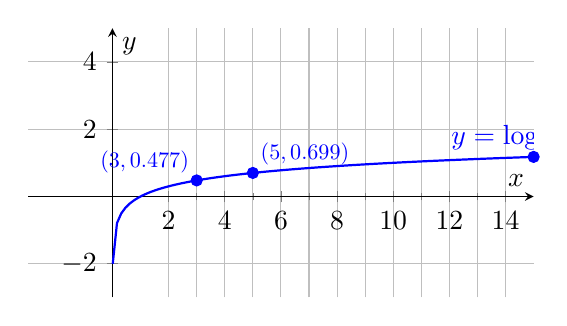
\begin{tikzpicture}
\begin{axis}[
    width=8cm, height=5cm,
    axis lines=middle,
    xmin=-3, xmax=15,
    ymin=-3, ymax=5,
    xtick={2,4,6,8,10,12,14},
    ytick={-2,2,4},
    xlabel={$x$},
    ylabel={$y$},
    grid=both,
    minor tick num=1,
    enlargelimits=false
]
\addplot[domain=0.01:15, samples=100, blue, thick] {log10(x)} node[pos=0.8, above right] {$y = \log x$};
\addplot[mark=*, blue] coordinates {(3,0.477)} node[above left, scale=0.8] {$(3, 0.477)$};
\addplot[mark=*, blue] coordinates {(5,0.699)} node[above right, scale=0.8] {$(5, 0.699)$};
\addplot[mark=*, blue] coordinates {(15,1.176)} node[below right, scale=0.8] {$(15, 1.176)$};
\end{axis}
\end{tikzpicture}
\end{center}

\textbf{A.} Complete the table shown.
\begin{center}
\begin{tabular}{|c|c|c|c|}
\hline
\textbf{$x$} & 3 & 5 & 15 \\ \hline
\textbf{$\log x$} & & & \\ \hline
\end{tabular}
\end{center}

\textbf{B. Look for Relationships} What is the relationship between the numbers 3, 5, and 15? What is the relationship between the logarithms of 3, 5, and 15?

\textbf{C.} What is your prediction for the value of $\log 45$? $\log 75$? Explain.
\end{model-discuss}

\textbf{ESSENTIAL QUESTION} How are the properties of logarithms used to simplify expressions and solve logarithmic equations?

\begin{concept-box}
\textbf{CONCEPT Properties of Logarithms}

For positive numbers $b$, $m$, and $n$ with $b \neq 1$, the following properties hold.

\begin{tabular}{ll}
Product Property of Logarithms & $\log_b{mn} = \log_b{m} + \log_b{n}$ \\
Quotient Property of Logarithms & $\log_b{\frac{m}{n}} = \log_b{m} - \log_b{n}$ \\
Power Property of Logarithms & $\log_b{m^n} = n\log_b{m}$
\end{tabular}
\end{concept-box}

\vspace{1em}
\textbf{LEARN TOGETHER}
How do you listen actively as others share ideas?

\begin{example}{1}
\textbf{Prove a Property of Logarithms}

\textbf{How can you prove the Product Property of Logarithms?}

Let $x = \log_b{m}$ and $y = \log_b{n}$. Then $b^x = m$ and $b^y = n$.
\begin{align*}
b^x \cdot b^y &= m \cdot n \quad \text{Multiply the expressions } b^x \text{ and } b^y. \\
b^{x+y} &= mn \\
x + y &= \log_b{mn} \quad \text{Rewrite the equation in logarithmic form.} \\
\log_b{m} + \log_b{n} &= \log_b{mn}
\end{align*}
\end{example}

\begin{tryit}{1}
Prove the Quotient Property of Logarithms.
\answer{Let $x = \log_b m$ and $y = \log_b n$. Then $b^x = m$ and $b^y = n$. $\frac{b^x}{b^y} = \frac{m}{n} \implies b^{x-y} = \frac{m}{n} \implies \log_b\left(\frac{m}{n}\right) = x - y \implies \log_b\left(\frac{m}{n}\right) = \log_b m - \log_b n$.}
\end{tryit}

\vspace{1em}
\textbf{MAKE SENSE AND PERSEVERE}
Expanding logarithmic expressions requires the use of a variety of properties. Look at the whole expression first to determine the sequence of properties that will be used.

\begin{example}{2}
\textbf{Expand Logarithmic Expressions}

\textbf{How can you use the properties of logarithms to expand each expression?}

\textbf{A.} $\log_5(a^2b^7)$
\begin{align*}
\log_5(a^2b^7) &= \log_5(a^2) + \log_5(b^7) \\
&= 2\log_5 a + 7\log_5 b
\end{align*}

\textbf{B.} $\ln\left(\frac{25}{3}\right)$
\begin{align*}
\ln\left(\frac{25}{3}\right) &= \ln\left(\frac{5^2}{3}\right) \\
&= \ln(5^2) - \ln 3 \\
&= 2\ln 5 - \ln 3
\end{align*}
\end{example}

\begin{tryit}{2}
Use the properties of logarithms to expand each expression.
\textbf{a.} $\log_7\left(\frac{r^3 t^4}{v}\right)$ \quad
\textbf{b.} $\ln\left(\frac{7}{225}\right)$
\answer{a. $3\log_7 r + 4\log_7 t - \log_7 v$ \quad b. $\ln 7 - 2\ln 15$}
\end{tryit}

\vspace{1em}
\textbf{STUDY TIP}
Recall that the Properties of Logarithms are each associated with a different operation. Addition signals the Product Property, subtraction signals the Quotient Property, and multiplication by a constant signals the Power Property.

\begin{example}{3}
\textbf{Write Expressions as Single Logarithms}

\textbf{What is each expression written as a single logarithm?}

\textbf{A.} $4\log_4 m + 3\log_4 n - \log_4 p$
\begin{align*}
4\log_4 m + 3\log_4 n - \log_4 p &= \log_4(m^4) + \log_4(n^3) - \log_4 p \\
&= \log_4(m^4 n^3) - \log_4 p \\
&= \log_4\left(\frac{m^4 n^3}{p}\right)
\end{align*}

\textbf{B.} $3\ln 2 - 2\ln 5$
\begin{align*}
3\ln 2 - 2\ln 5 &= \ln(2^3) - \ln(5^2) \\
&= \ln\left(\frac{2^3}{5^2}\right) \\
&= \ln\left(\frac{8}{25}\right)
\end{align*}
\end{example}

\begin{tryit}{3}
Write each expression as a single logarithm.
\textbf{a.} $5\log_2 c - 7\log_2 n$ \quad
\textbf{b.} $2\ln 7 + \ln 2$
\answer{a. $\log_2\left(\frac{c^5}{n^7}\right)$ \quad b. $\ln 98$}
\end{tryit}

\vspace{1em}
\textbf{APPLICATION}

\begin{example}{4}
\textbf{Apply Properties of Logarithms}

\placeholder{diagram}{A graphical chart showing pH levels for different solutions: Orange juice (pH = 3), Acid rain (pH = 4.5), Clear rain (pH = 5.6), and Healthy lake (pH = 6.5).}

The pH of a solution is a measure of its concentration of hydrogen ions. This concentration (measured in moles per liter) is written $[H^+]$ and is given by the formula
\[ \text{pH} = \log\frac{1}{[H^+]}. \]

\textbf{What is the concentration of hydrogen ions in the acid rainfall?}

Solve for $[H^+]$
\begin{align*}
4.5 &= \log\frac{1}{[H^+]} \\
4.5 &= \log 1 - \log[H^+] \\
-4.5 &= \log[H^+] \\
10^{-4.5} &= [H^+]
\end{align*}
The concentration of hydrogen ions in the acid rainfall is $10^{-4.5} \approx 0.0000316$ moles per liter.

\textbf{COMMON ERROR}
The expression $\log\frac{1}{[H^+]}$ is equal to $\log 1 - \log[H^+]$, not $\log[1 - H^+]$.
\end{example}

\begin{tryit}{4}
What is the concentration of hydrogen ions in a liter of orange juice?
\answer{$10^{-3} = 0.001$ moles per liter}
\end{tryit}

\vspace{1em}
\textbf{CONCEPTUAL UNDERSTANDING}

\textbf{STUDY TIP}
To divide logs with a calculator using one expression, be sure to include parentheses in the correct places. To evaluate $\log_2 3$, press [LOG] [3] [$\div$] [(] [LOG] [2] [)] [ENTER.]

\begin{example}{5}
\textbf{Evaluate Logarithmic Expressions by Changing the Base}

\textbf{How can you use base 10 logarithms to evaluate base 2 logarithms?}

To evaluate $\log_2 3$ with a calculator, you need to express $\log_2 3$ in terms of base 10 logarithms.

\begin{align*}
\log_2 3 &= \frac{\log_2 3 \cdot \log 2}{\log 2} \\
&= \frac{\log 2^{\log_2 3}}{\log 2} \quad \text{Remember that exponents and logarithms are inverse operations, so they undo one another.} \\
&= \frac{\log 3}{\log 2} \\
&\approx \frac{0.477}{0.301} \approx 1.585
\end{align*}

This illustrates the \textbf{Change of Base Formula}:

For positive numbers $m$, $b$, and $a$, with $b \neq 1$ and $a \neq 1$, $\log_b m = \frac{\log_a m}{\log_a b}$.
\end{example}

\begin{tryit}{5}
Estimate the value of each logarithm. Then use a calculator to find the value of each logarithm to the nearest thousandth.
\textbf{a.} $\log_2 7$ \quad
\textbf{b.} $\log_5 3$
\answer{a. $\approx 2.807$ \quad b. $\approx 0.683$}
\end{tryit}

\vspace{1em}
\textbf{STUDY TIP}
The equation $2^x = 7$ can also be solved using natural logarithms.

\begin{example}{6}
\textbf{Use the Change of Base Formula}

\textbf{What is the solution of the equation $2^x = 7$? Express the solution as a logarithm and then evaluate. Round to the nearest thousandth.}
\begin{align*}
2^x &= 7 \\
x &= \log_2 7 \\
x &= \frac{\log 7}{\log 2} \\
x &\approx 2.807
\end{align*}
Check $2^{2.807} \approx 7$
\end{example}

\begin{tryit}{6}
What is the solution to the equation $3^x = 15$? Express the solution as a logarithm, make an estimate, and then evaluate. Round to the nearest thousandth.
\answer{$x = \log_3 15 \approx 2.465$}
\end{tryit}

\begin{concept-summary}
\textbf{CONCEPT SUMMARY Properties of Logarithms}

\begin{center}
\renewcommand{\arraystretch}{1.5}
\begin{tabular}{lp{3cm}p{3cm}p{3cm}p{3cm}}
\toprule
& \textbf{Product Property} & \textbf{Quotient Property} & \textbf{Power Property} & \textbf{Change of Base} \\
\midrule
\textbf{ALGEBRA} & $\log_b(mn) =$ \newline $\log_b m + \log_b n$ & $\log_b\left(\frac{m}{n}\right) =$ \newline $\log_b m - \log_b n$ & $\log_b(m^n) =$ \newline $n \cdot \log_b m$ & $\log_b m = \frac{\log_a m}{\log_a b}$ \\
\midrule
\textbf{WORDS} & The log of a product is the sum of the logs. & The log of a quotient is the difference of the logs. & The log of a number raised to a power is the power multiplied by the log of the number. & The log base $b$ of a number is equal to the log base $a$ of the number divided by the log base $a$ of $b$. \\
\midrule
\textbf{NUMBERS} & $\log_2(20) =$ \newline $\log_2(4) + \log_2(5)$ & $\log_{10}\left(\frac{2}{3}\right) =$ \newline $\log_{10} 2 - \log_{10} 3$ & $\log_3(16) = 4 \cdot \log_3 2$ & $\log_5 7 = \frac{\log 7}{\log 5}$ \\
\bottomrule
\end{tabular}
\end{center}
\end{concept-summary}

\vspace{1em}
\textbf{Do You UNDERSTAND?}
\begin{enumerate}
    \item \textbf{ESSENTIAL QUESTION} How are the properties of logarithms used to simplify expressions and solve logarithmic equations?
    \item \textbf{Vocabulary} While it is not necessary to change to base 10 when applying the Change of Base Formula, why is it common to do so?
    \item \textbf{Error Analysis} Amanda claimed the expanded form of the expression $\log_4(c^2 d^5)$ is $5\log_4 c + 5\log_4 d$. Explain the error Amanda made.
\end{enumerate}

\textbf{Do You KNOW HOW?}
\begin{enumerate}
    \setcounter{enumi}{3}
    \item Use the properties of logarithms to expand the expression $\log_6\left(\frac{49}{5}\right)$.
    \item Use the properties of logarithms to write the expression $5\ln s + 6\ln t$ as a single logarithm.
    \item Use the formula $\text{pH} = \log\frac{1}{[H^+]}$ to write an expression for the concentration of hydrogen ions, $[H^+]$, in a container of baking soda with a pH of 8.9.
\end{enumerate}


\section*{PRACTICE \& PROBLEM SOLVING}

\textbf{UNDERSTAND}

\begin{practice}{7}{}
\textbf{Use Structure} Without applying the Change of Base Formula, explain how to use $\log_3 2 \approx 0.631$ and $\log_3 5 \approx 1.465$ to approximate $\log_3\left(\frac{2}{5}\right)$.
\answer{$\log_3\left(\frac{2}{5}\right) = \log_3 2 - \log_3 5 \approx 0.631 - 1.465 = -0.834$}
\end{practice}

\begin{practice}{8}{}
\textbf{Communicate Precisely} Explain what is meant by expanding a logarithmic expression. How are the processes of expanding logarithmic expressions and writing logarithmic expressions as a single logarithm related?
\answer{They are inverse processes using the same properties in reverse directions.}
\end{practice}

\begin{practice}{9}{}
\textbf{Higher Order Thinking} The graph of $y = \log\left(\frac{1}{x}\right)$ and $y = -\log x$ are shown. Notice the graph is the same for both equations. Use properties of logarithms to explain why the graphs are the same.

\begin{center}
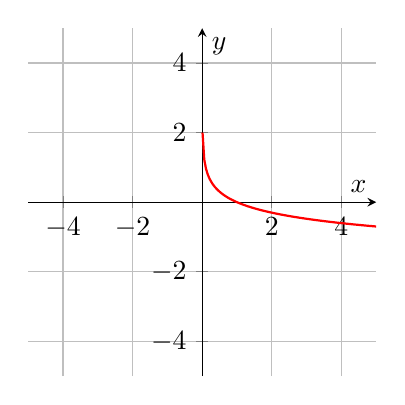
\begin{tikzpicture}
\begin{axis}[
    width=6cm, height=6cm,
    axis lines=middle,
    xmin=-5, xmax=5,
    ymin=-5, ymax=5,
    xtick={-4,-2,2,4},
    ytick={-4,-2,2,4},
    xlabel={$x$},
    ylabel={$y$},
    grid=both
]
\addplot[domain=0.01:5, samples=100, red, thick] {-log10(x)};
\end{axis}
\end{tikzpicture}
\end{center}
\answer{$\log\left(\frac{1}{x}\right) = \log(x^{-1}) = -1 \log(x) = -\log x$}
\end{practice}

\begin{practice}{10}{}
\textbf{Communicate Precisely} Saachi used the Change of Base Formula to solve the equation $6^x = 72$ and found that $x = 2.387$. How can Saachi check her solution?
\answer{Evaluate $6^{2.387}$ and see if it is approximately 72.}
\end{practice}

\begin{practice}{11}{}
\textbf{Error Analysis} Describe and correct the error a student made in writing the logarithmic expression in terms of a single logarithm.

$\log_3 2 + \frac{1}{2}\log_3 y = \log_3 2y^2$ \quad [Incorrect]
\answer{The student brought the exponent in incorrectly. It should be $y^{1/2}$, not $y^2$. The correct expression is $\log_3(2\sqrt{y})$.}
\end{practice}

\begin{practice}{12}{}
\textbf{Error Analysis} A student wants to approximate $\log_2 9$ with her calculator. She enters the equivalent expression $\frac{\ln 2}{\ln 9}$, but the decimal value is not close to her estimate of 3. What happened?

$\log_2 9 = \frac{\ln 2}{\ln 9}$ \quad [Incorrect]
\answer{The student divided the log of the base by the log of the number. The Change of Base Formula gives $\frac{\ln 9}{\ln 2}$.}
\end{practice}

\vspace{1em}
\textbf{PRACTICE}

\begin{practice}{13}{}
Use the properties of exponents to prove the Power Property of Logarithms. SEE EXAMPLE 1
\answer{Let $x = \log_b m$, so $b^x = m$. Then $m^n = (b^x)^n = b^{nx}$. Therefore, $\log_b(m^n) = nx = n\log_b m$.}
\end{practice}

Use the properties of logarithms to expand each expression. SEE EXAMPLE 2
\begin{practice}{14}{}
$\log_5\left(\frac{2}{3}\right)$
\answer{$\log_5 2 - \log_5 3$}
\end{practice}

\begin{practice}{15}{}
$\log_6(2 m^5 n^3)$
\answer{$\log_6 2 + 5\log_6 m + 3\log_6 n$}
\end{practice}

\begin{practice}{16}{}
$\ln 2x^5$
\answer{$\ln 2 + 5\ln x$}
\end{practice}

\begin{practice}{17}{}
$\log_2\left(\frac{x}{5y}\right)$
\answer{$\log_2 x - \log_2 5 - \log_2 y$}
\end{practice}

Use the properties of logarithms to write each expression as a single logarithm. SEE EXAMPLE 3
\begin{practice}{18}{}
$9\ln x - 6\ln y$
\answer{$\ln\left(\frac{x^9}{y^6}\right)$}
\end{practice}

\begin{practice}{19}{}
$\log_5 6 + \frac{1}{2}\log_5 y$
\answer{$\log_5(6\sqrt{y})$}
\end{practice}

\begin{practice}{20}{}
$2\log 10 + 4\log(3x)$
\answer{$\log(8100x^4)$}
\end{practice}

\begin{practice}{21}{}
$\frac{1}{3}\ln 27 - 3\ln(2y)$
\answer{$\ln\left(\frac{3}{8y^3}\right)$}
\end{practice}

\begin{practice}{22}{}
$8\log_3 2 + 5\log_3 c + 7\log_3 d$
\answer{$\log_3(256c^5 d^7)$}
\end{practice}

\begin{practice}{23}{}
Use properties of logarithms to show that $\text{pH} = \log\frac{1}{[H^+]}$ can be written as $\text{pH} = -\log[H^+]$. SEE EXAMPLE 4
\answer{$\log\left(\frac{1}{[H^+]}\right) = \log 1 - \log[H^+] = 0 - \log[H^+] = -\log[H^+]$.}
\end{practice}

Use the Change of Base Formula to evaluate each logarithm. Round to the nearest thousandth. SEE EXAMPLE 5
\begin{practice}{24}{}
$\log_4 9$
\answer{$1.585$}
\end{practice}

\begin{practice}{25}{}
$\log_6 5$
\answer{$0.898$}
\end{practice}

\begin{practice}{26}{}
$\ln 3$
\answer{$1.099$}
\end{practice}

\begin{practice}{27}{}
$\log_2 7$
\answer{$2.807$}
\end{practice}

\begin{practice}{28}{}
$\log_9 12$
\answer{$1.131$}
\end{practice}

\begin{practice}{29}{}
$\ln 23$
\answer{$3.135$}
\end{practice}

Use the Change of Base Formula to solve each equation for $x$. Give an exact solution as a logarithm and an approximate solution rounded to the nearest thousandth. SEE EXAMPLE 6
\begin{practice}{30}{}
$3^x = 4$
\answer{$x = \log_3 4 \approx 1.262$}
\end{practice}

\begin{practice}{31}{}
$5^x = 11$
\answer{$x = \log_5 11 \approx 1.490$}
\end{practice}

\begin{practice}{32}{}
$8^x = 10$
\answer{$x = \log_8 10 \approx 1.107$}
\end{practice}

\begin{practice}{33}{}
$2^x = 30$
\answer{$x = \log_2 30 \approx 4.907$}
\end{practice}

\begin{practice}{34}{}
$7^x = 100$
\answer{$x = \log_7 100 \approx 2.367$}
\end{practice}

\begin{practice}{35}{}
$4^x = 55$
\answer{$x = \log_4 55 \approx 2.891$}
\end{practice}


\vspace{1em}
\textbf{APPLY}

\begin{practice}{36}{}
\textbf{Make Sense and Persevere} The loudness of sound is measured in decibels. For a sound with intensity $I$ (in watts per square meter), its loudness $L(I)$ (in decibels) is modeled by the function $L(I) = 10\log\frac{I}{I_0}$, where $I_0$ represents the intensity of a barely audible sound (approximately $10^{-12}$ watts per square meter).

\placeholder{photo}{Illustration of cars in heavy traffic (label: Heavy Traffic: intensity of $I = 10^{-4}$ watts per square meter) and a boy listening to music through headphones (label: Music through headphones: 40 dB).}

\textbf{a.} Find the decibel level of the sound made by the heavy traffic.
\answer{$80$ dB}

\textbf{b.} Find the intensity of the sound that is made by music playing at 40 decibels.
\answer{$10^{-8}$ watts per square meter}

\textbf{c.} How many times as great is the intensity of the traffic than the intensity of the music?
\answer{$10,000$ times}
\end{practice}

\begin{practice}{37}{}
\textbf{Model with Mathematics} Miguel collected data on the attendance at an amusement park and the daily high temperature. He found that the model $A = 2\log t + \log 5$ approximated the attendance $A$, in thousands of people, at the amusement park, when the daily high temperature is $t$ degrees Fahrenheit.

\textbf{a.} Use properties of logarithms to simplify Miguel's formula.
\answer{$A = \log(5t^2)$}

\textbf{b.} The daily high temperatures for the week are below.

\begin{center}
\begin{tabular}{ccccc}
Mon & Tue & Wed & Thu & Fri \\
87°/66° & 73°/67° & 65°/61° & 72°/57° & 80°/59° \\
\end{tabular} \\
\footnotesize Daily temperatures show highs and lows in °F.
\end{center}

What is the expected attendance on Wednesday? Round to the nearest person.
\answer{$A = \log(5 \cdot 65^2) \approx 4.325$ thousand $\implies 4,325$ people}
\end{practice}

\vspace{1em}
\textbf{ASSESSMENT PRACTICE}

\begin{practice}{38}{}
Select all the expressions equal to $\log_2 3$.
\begin{itemize}
    \item[$\square$] $\frac{\log 3}{\log 2}$
    \item[$\square$] $\frac{\log 2}{\log 3}$
    \item[$\square$] $\frac{\log_2 3}{\log_2 2}$
    \item[$\square$] $\frac{\log_3 2}{\log_3 3}$
    \item[$\square$] $\frac{\log_3 3}{\log_3 2}$
\end{itemize}
\answer{Select options 1, 3, and 5.}
\end{practice}

\begin{practice}{39}{}
\textbf{SAT/ACT} Use the properties of logarithms to write the following expression in terms of a single logarithm.
\[ 2(\log_3 20 - \log_3 4) + 0.5 \log_3 4 \]
\begin{itemize}
    \item[A] $\log_3 4$
    \item[B] $\log_3 5$
    \item[C] $\log_3 25$
    \item[D] $\log_3 50$
\end{itemize}
\answer{D}
\end{practice}

\begin{practice}{40}{}
\textbf{Performance Task} The magnitude, or intensity, of an earthquake is measured on the Richter scale. For an earthquake where the amplitude of its seismographic trace is $A$, its magnitude is modeled by the function:
\[ R(A) = \log\frac{A}{A_0}, \]
where $A_0$ represents the amplitude of the smallest detectable earthquake.

\textbf{Part A} An earthquake occurs with an amplitude 200 times greater than the amplitude of the smallest detectable earthquake, $A_0$. What is the magnitude of this earthquake on the Richter scale?
\answer{$\approx 2.3$}

\textbf{Part B} Approximately how many times as great is the amplitude of an earthquake measuring 6.8 on the Richter scale than the amplitude of an earthquake measuring 5.9 on the Richter scale?
\answer{$\approx 7.94$ times}

\textbf{Part C} Suppose the intensity of one earthquake is 150 times as great as that of another. How much greater is the magnitude of the more intense earthquake than the less intense earthquake?
\answer{$\approx 2.18$ greater on the Richter scale}
\end{practice}

\end{document}